\documentclass[12pt,]{article}
\usepackage{lmodern}
\usepackage{amssymb,amsmath}
\usepackage{ifxetex,ifluatex}
\usepackage{fixltx2e} % provides \textsubscript
\ifnum 0\ifxetex 1\fi\ifluatex 1\fi=0 % if pdftex
  \usepackage[T1]{fontenc}
  \usepackage[utf8]{inputenc}
\else % if luatex or xelatex
  \ifxetex
    \usepackage{mathspec}
  \else
    \usepackage{fontspec}
  \fi
  \defaultfontfeatures{Ligatures=TeX,Scale=MatchLowercase}
\fi
% use upquote if available, for straight quotes in verbatim environments
\IfFileExists{upquote.sty}{\usepackage{upquote}}{}
% use microtype if available
\IfFileExists{microtype.sty}{%
\usepackage{microtype}
\UseMicrotypeSet[protrusion]{basicmath} % disable protrusion for tt fonts
}{}
\usepackage[margin=1in]{geometry}
\usepackage{hyperref}
\hypersetup{unicode=true,
            pdftitle={Final Project-Research Article},
            pdfborder={0 0 0},
            breaklinks=true}
\urlstyle{same}  % don't use monospace font for urls
\usepackage{longtable,booktabs}
\usepackage{graphicx,grffile}
\makeatletter
\def\maxwidth{\ifdim\Gin@nat@width>\linewidth\linewidth\else\Gin@nat@width\fi}
\def\maxheight{\ifdim\Gin@nat@height>\textheight\textheight\else\Gin@nat@height\fi}
\makeatother
% Scale images if necessary, so that they will not overflow the page
% margins by default, and it is still possible to overwrite the defaults
% using explicit options in \includegraphics[width, height, ...]{}
\setkeys{Gin}{width=\maxwidth,height=\maxheight,keepaspectratio}
\IfFileExists{parskip.sty}{%
\usepackage{parskip}
}{% else
\setlength{\parindent}{0pt}
\setlength{\parskip}{6pt plus 2pt minus 1pt}
}
\setlength{\emergencystretch}{3em}  % prevent overfull lines
\providecommand{\tightlist}{%
  \setlength{\itemsep}{0pt}\setlength{\parskip}{0pt}}
\setcounter{secnumdepth}{0}
% Redefines (sub)paragraphs to behave more like sections
\ifx\paragraph\undefined\else
\let\oldparagraph\paragraph
\renewcommand{\paragraph}[1]{\oldparagraph{#1}\mbox{}}
\fi
\ifx\subparagraph\undefined\else
\let\oldsubparagraph\subparagraph
\renewcommand{\subparagraph}[1]{\oldsubparagraph{#1}\mbox{}}
\fi

%%% Use protect on footnotes to avoid problems with footnotes in titles
\let\rmarkdownfootnote\footnote%
\def\footnote{\protect\rmarkdownfootnote}

%%% Change title format to be more compact
\usepackage{titling}

% Create subtitle command for use in maketitle
\providecommand{\subtitle}[1]{
  \posttitle{
    \begin{center}\large#1\end{center}
    }
}

\setlength{\droptitle}{-2em}

  \title{Final Project-Research Article}
    \pretitle{\vspace{\droptitle}\centering\huge}
  \posttitle{\par}
  \subtitle{Research Article}
  \author{David Sun, Elizabeth Morales, Jaehee Jeong\\
Sarah Heuschele, Tyler Chun, Yolanda Jin\\[2\baselineskip]Team Name: i
need a \textless{}/br\textgreater{}}
    \preauthor{\centering\large\emph}
  \postauthor{\par}
      \predate{\centering\large\emph}
  \postdate{\par}
    \date{6/1/2021}

\usepackage{wrapfig}
\usepackage{lipsum}

\begin{document}
\maketitle

{
\setcounter{tocdepth}{2}
\tableofcontents
}
The research report focuses on the benefits of colic surgery for horses
that are admitted into the hospital for abdominal issues. Colic surgery
is used to treat issues that affect the longevity of a horse, most
commonly used to address issues within the gastrointestinal tract. The
data gave us a look into 299 hospital cases of horses that were admitted
due to poor health, and of those horses which lived, died, or were
euthanized. The data also provided an indicator to whether the horse
received surgery or not. Our analysis focused on looking at the horses
admitted and their outcome. From there, we wanted to explore the key
characteristics of the horse's condition to determine if the outcome
could have been different had they received surgery, especially the
horses that had symptoms related to Colic Surgery.``)

\begin{wrapfigure}{R}{0.6\textwidth}

\hfill{}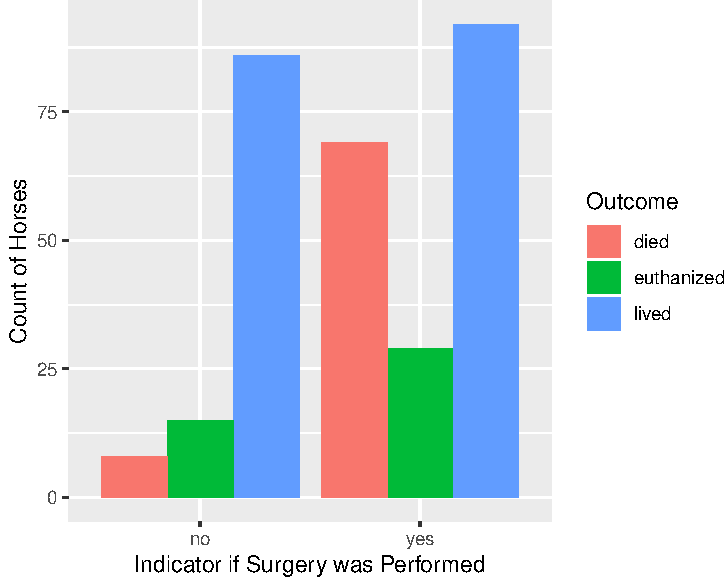
\includegraphics[width=.7\textwidth]{Final_Project_-_Executive_Summary_files/figure-latex/unnamed-chunk-4-1} 

\caption{Horse Outcome vs Surgery Performed}\label{fig:unnamed-chunk-4}
\end{wrapfigure}

This analysis is proved useful in determining if colic surgery can be
beneficial in saving a horse's life when admitted into the hospital. Our
initial hypothesis was that the increase in surgeries to treat
gastrointestinal tract complications in horses would lead to an increase
in the number of horses that lived.

With the data given, we explored the different components of a horse's
health, focusing primarily on their gastrointestinal tract. A few of the
key factors were the horse's protein levels, pH levels and rectal
temperature.

From our initial analysis, we found that while the number of horses that
lived did not change much between horses who had surgery and those who
did not, the number of horse that died after surgery grew by about 3
times the amount of those without surgery.

Based on this discovery, we wanted to explore the correlation what
brought the horse to the hospital, if they received surgery, and how
that affected the outcome. The data provided insight on whether the
horse entered the hospital due to something that was deemed ``worthy of
surgery.'' We used this in conjunction with if the horse actually
received surgery to expand on the hypothesis that horses that need
surgery, and receive surgery, are more likely to live.

\begin{longtable}[]{@{}llrrr@{}}
\toprule
Was it Surgical? & Did They Have Surgery & Died & Euthanized &
Lived\tabularnewline
\midrule
\endhead
no & no & 6 & 5 & 75\tabularnewline
no & yes & 2 & 10 & 11\tabularnewline
yes & no & 13 & 12 & 8\tabularnewline
yes & yes & 56 & 17 & 84\tabularnewline
\bottomrule
\end{longtable}

\textbf{THIS PARAGRAPH IS COPY AND PAST FROM THE OTHER REPORT IT NEEDS
TO BE RE WORDED} From the horse demographics, we have found that even
though there is a very small number of young horses, there is a higher
``lived'' adult horse proportion than young horses. This might be due to
adult horses having more robust health system to recover from surgeries
and illness. Horse's hospital demographics show that if a horse was to
return to the hospital, they had a 20\% higher chance of being
euthanized or dying. Those who lived have three times higher proportions
(around 60\%) of normal and warm temperatures than those who died or
euthanized (18\textasciitilde{}20\%). About 70\% of lived horses had
normal peripheral pulse and about 70\% of died or euthanized horses had
problematic peripheral pulses. The distribution for lived horses had
more stable rectal temperatures than the other two groups. About 60\% of
the lived horses had normal circulation when about
20\textasciitilde{}25\% of the died or euthanized horses had normal
circulation. This two way table states that the more pain a horse has,
it is less likely to be ``lived'' than ``died'' or ``euthanized''.


\end{document}
